\documentclass{report}
\usepackage[utf8]{inputenc}
\usepackage{hyperref}

\title{Proyecto 1 de Redes de Computadoras}
\author{Arteaga Hernández Alejandro Iabin\\
Barocio Gómez Luis Fernando\\
Olea Olvera Marco Iván}
\date{Octubre 2019}
\usepackage{natbib}
\usepackage{graphicx}
\begin{document}

% Subtract 1 from counters that are used
\renewcommand{\thesection}{\thechapter.\number\numexpr\value{section}-1\relax}
\renewcommand{\thesubsection}{\thesection.\number\numexpr\value{subsection}-1\relax}
\renewcommand{\thesubsubsection}{\thesubsection.\number\numexpr\value{subsubsection}-1\relax}
\setcounter{secnumdepth}{3}
\setcounter{chapter}{1}

\maketitle

\section{Diagrama de red}

\begin{figure}[h!]
    \centering
    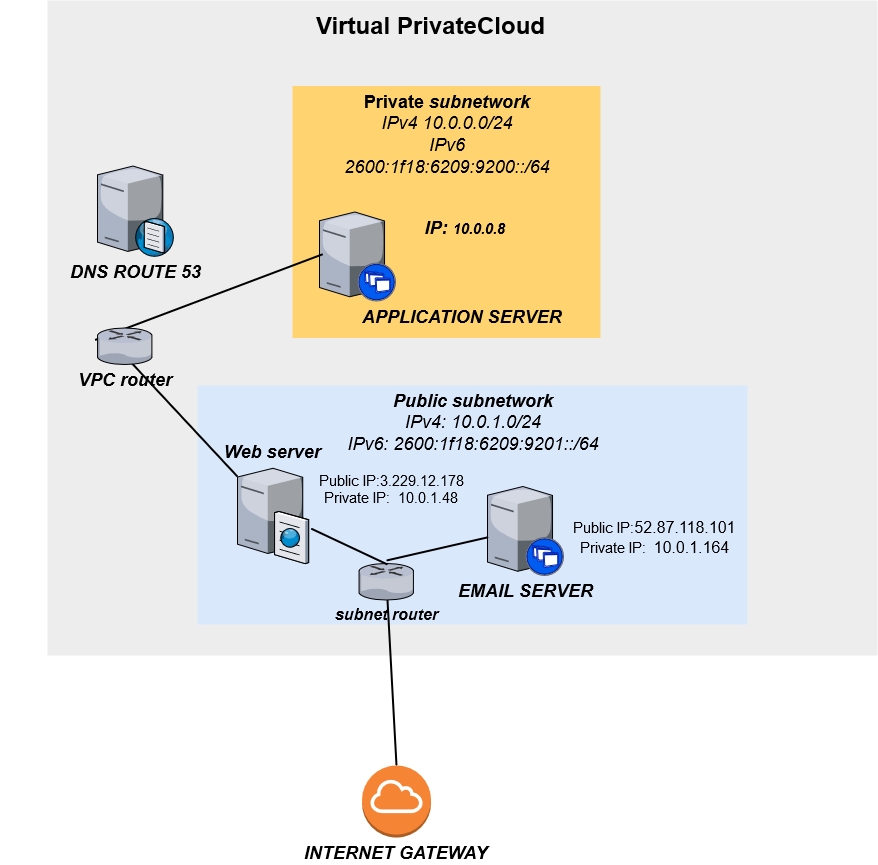
\includegraphics[scale=0.5]{diag}
    \caption{Diagrama de red}
\end{figure}


\section{Registros DNS}

Registros DNS usados para nuestra Virtual Private Cloud usando el servicio Route 53:
\begin{center}
\begin{tabular}{ |c|c|c| }
\hline
TYPE & NAME & CONTENT \\ 
\hline
A & app.proyectoredes.tk & 10.0.0.8  \\ 
A & mail.proyectoredes.tk & 10.0.1.164 \\
A & web.proyectoredes.tk & 10.0.1.48 \\
CNAME & www.proyectoredes.tk & proyectoredes.tk \\
CNAME & site.proyectoredes.tk & app.proyectoredes.tk \\
MX & proyectoredes.tk & mail.proyectoredes.tk \\
\hline
\end{tabular}
\end{center}

Registros DNS usados para nuestro dominio usando el servicio de CloudFlare:

% \begin{center}
% \begin{tabular}{ |c|c|c| }
% \hline
% TYPE & NAME & CONTENT \\ 
% \hline
% A & proyectoredes.tk & 3.229.12.178  \\ 
% A & mail.proyectoredes.tk & 52.87.118.101 \\
% AAAA & proyectoredes.tk & 2600:1f18:6209:9201:9b35:8d53:4043:ab2e \\
% AAAA & mail.proyectoredes.tk & 2600:1f18:6209:9201:8062:1512:16a0:2178 \\
% CNAME & www.proyectoredes.tk & proyectoredes.tk \\
% MX & proyectoredes.tk & mail.proyectoredes.tk \\
% PTR & mail.proyectoredes.tk & 101.118.87.52.in-addr.arpa \\
% PTR & mail.proyectoredes.tk & 8.7.1.2.0.a.6.1.2.1.5.1.2.6.0.8.1.0.2.9.9.0.2.6.8.1.f.1.0.0.6.2.ip6.arpa \\
% TXT & proyectoredes.tk & v=spf1 mx include:\_spf.google.com -all \\
% TXT & \_dmarc.proyectoredes.tk & v=DMARC1; p=reject; rua=mailto:admin@proyectoredes.tk; \\
% & & ruf=mailto:admin@proyectoredes.tk; fo=1; rf=afrf; pct=100 \\
% TXT & mail.\_domainkey & v=DKIM1; h=sha256; k=rsa; \\
% & .proyectoredes.tk & p=\{llave pública omitida por brevedad\}\\
% \hline
% \end{tabular}
% \end{center}

\begin{figure}[h!]
    \centering
    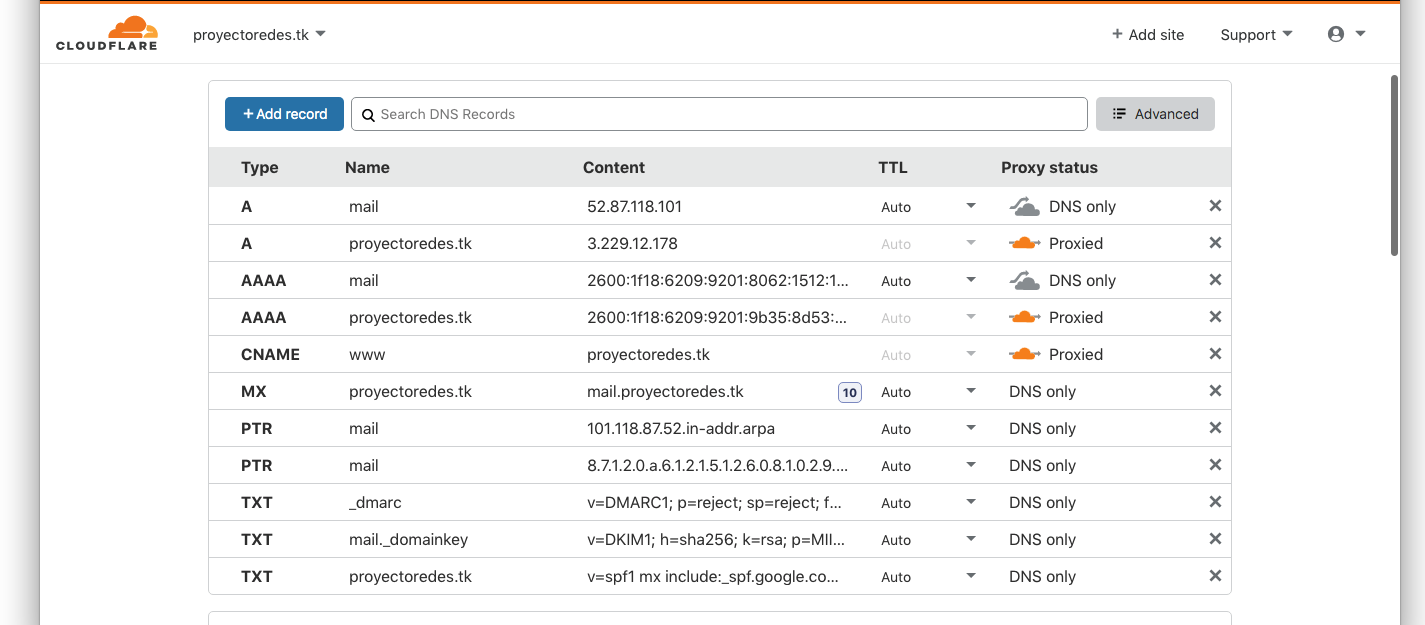
\includegraphics[scale=0.3]{cloudflare.png}
    \caption{CloudFlare}
\end{figure}

\section{Resúmenes de las configuraciones}

\subsection{Servidor web}
Para el servidor web, decidimos usar un servidor Apache. Tenemos dos archivos de configuración principales. \\ \\
El primero recibe peticiones por el puerto 80 ya que es el default para HTTP. Lo que hace es recibir una petición con el dominio www.proyectoredes.tk o proyectoredes.tk y lo redirige hacía una nueva petición pero ahora usando el protocolo HTTPS.
\\
\begin{figure}[h!]
\centering
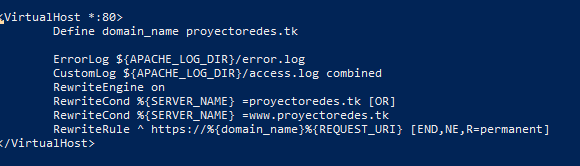
\includegraphics[scale=0.5]{Capture}
\caption{Configuración para el puerto 80}
\label{fig:web}
\end{figure}
\\
El segundo archivo de configuración es aquel que recibe las peticiones HTTPS a través del puerto 443.
Se cargan las dos llaves generadas por LetsEncrypt para certificar el contenido y la llave para cifrarlo, una vez que hemos hecho eso se configuró un reverse proxy, que redirige las peticiones recibidas por el puerto 443 hacía la dirección app.proyectoredes.tk ya que esa dirección es resuelta por el DNS de Route 53 hacía la IP del servidor de aplicación, entonces usando este reverse proxy redirigimos todo el tráfico hacía nuestro server de aplicación a el puerto 8080.\\
\begin{figure}
  \centering
\includegraphics[scale=0.4]{Capture2}
\caption{Configuración para el puerto 443}
    \label{fig:my_label}
\end{figure}
\\\\
Esto muestra la manera en la que especificamos el proxy inverso configurado en nuestro servidor web.\\\\

\subsection{Servidor de aplicación y base de datos}

El servidor de aplicación está configurado para ofrecer servicio a través del puerto 8080.
Usamos un framework de python llamado django.
Necesitamos expresar la IP de la EC2 en el servidor para que se pudieran hacer peticiones desde ahí y desde web.proyectoredes.tk,
dominio que es resuelto por el DNS hacía la IP local del servidor EC2 de aplicación.
Además en la configuración de django tuvimos que agregar la IP del servidor a los hosts permitidos.

La base de datos decidimos usar SQLite, pero django de ofrece una interfaz sencilla para conectarte a diversos manejadores de bases de datos. Si necesitáramos extender nuestra base de datos a otro servidor en la private subnetwork (así llamamos a nuestra red privada en VPC), simplemente tendríamos que especificar el driver del manejador, la dirección IP o el dominio local que deberíamos registrar en route 53 y el usuario y contraseña de la base.

\begin{figure}[h!]
    \centering
    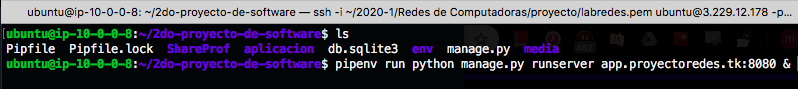
\includegraphics[scale=0.5]{django.png}
    \caption{Django}
\end{figure}

\subsection{Servidor de correo electrónico}

Para el servidor SMTPS usamos postfix. Copiamos a nuestro servidor mail las llaves generadas por certbot para implementar HTTPS en el servidor web. \\
En su configuración se especifican las direcciones que tienen permitidos enviar correos de nuestro dominio, para prevenir un open relay (variable \texttt{mynetworks}).

\begin{figure}[h!]
    \centering
    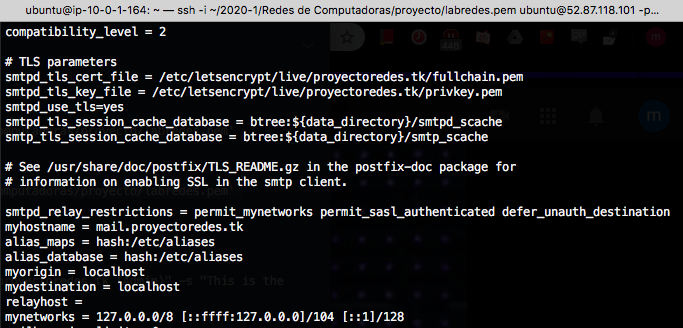
\includegraphics[scale=0.5]{mail/postfix.png}
    \caption{main.cf, archivo de configuración de postfix}
\end{figure}

Para los servidores POP3S y IMAPS utilizamos dovecot. Utiliza las mismas llaves que usamos para HTTPS y SMTPS y, al igual que nuestro servidor SMTPS, no utiliza los puertos especiales de conexión segura de POP3 y IMAP, funciona con STARTTLS. \\ 
Es decir, nuestro servidor de correo usa los puertos estándares 25, 110 y 143, pero con un protocolo de TLS oportunista. Para prevenir un ataque STRIPTLS se han habilitado opciones que rechazan conexiones que no tienen disponibles TLS (\texttt{-o smtpd\_tls\_security\_level=encrypt} en postfix y \texttt{ssl=required} en dovecot).

\begin{figure}[h!]
    \centering
    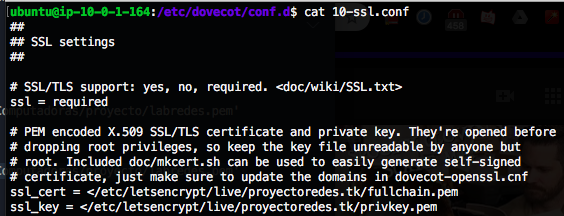
\includegraphics[scale=0.8]{mail/dovecot-ssl.png}
    \caption{Caption}
\end{figure}

Por último, configuramos el paquete opendkim, el cual firma correos que salen de nuestro dominio y servidor con nuestra llave DKIM. Esto se puede verificar en los headers de cualquier correo que sí haya sido enviado por nosotros.

\section{Esquema de la base de datos}

\begin{figure}[h!]
\centering
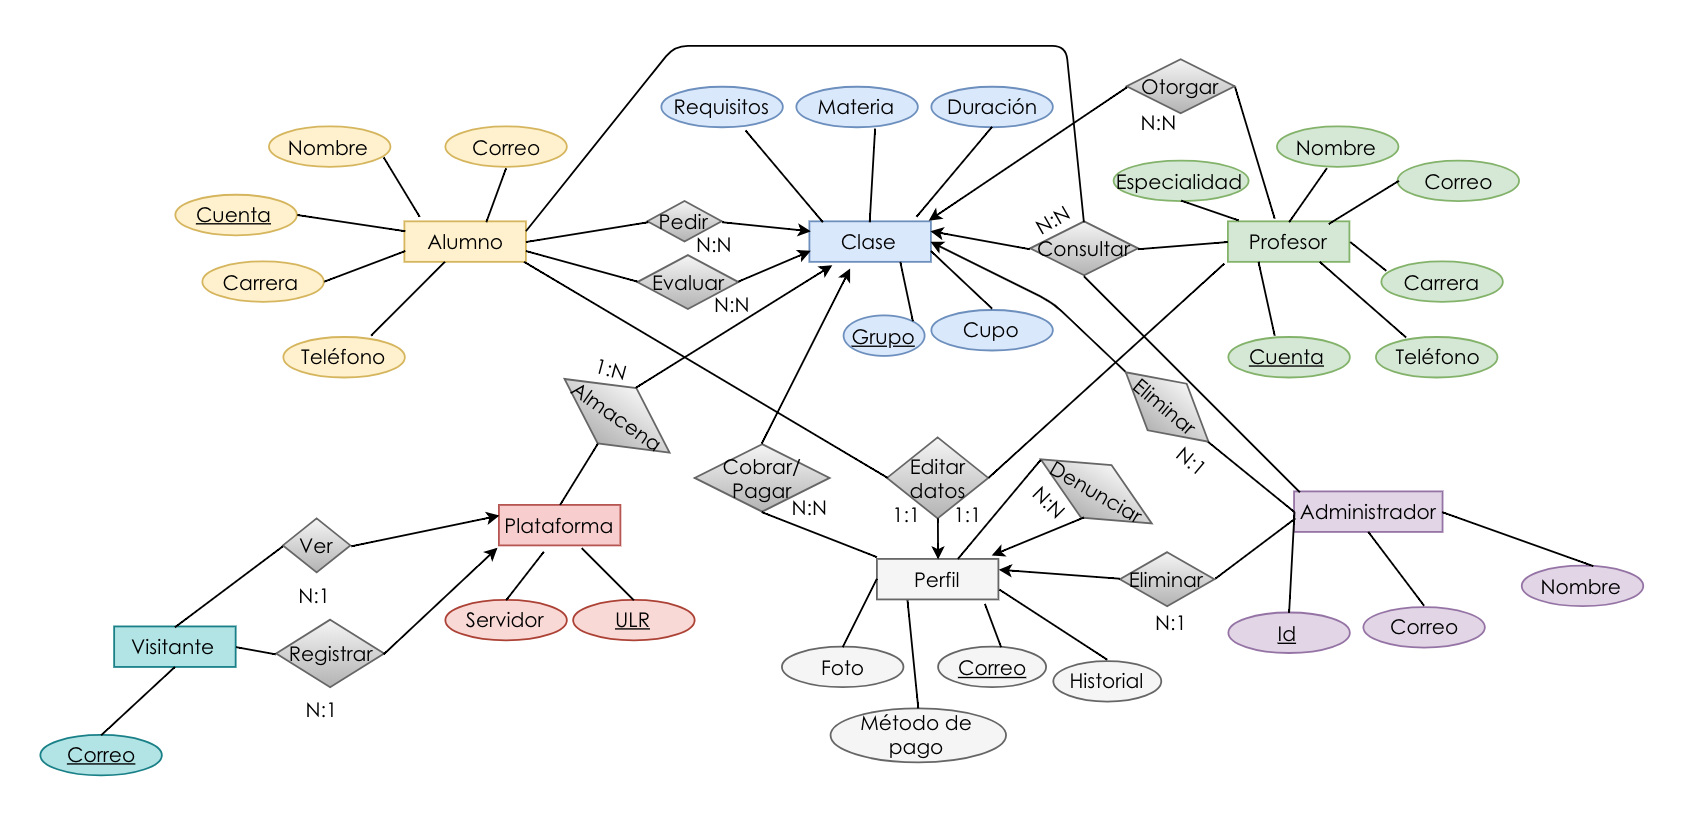
\includegraphics[scale=0.5]{db}
\caption{Diagrama relacional de la base de datos}
%\label{fig:universe}
\end{figure}

 \section{Objetivo de la aplicación}
Implementar una plataforma de economía compartida para relacionar profesores y alumnos. ~\\ ~\\
Alcance\\
\begin{itemize}
 \item Funciones generales:
\item Navegar
\item Registro 
\item Pedir clase
\item Manejo de sesión 
\item Calificar 
\item Comunicación entre profesor y alumno
\end{itemize}

Actores:
\begin{itemize}
\item Usuario
\item Visitante
\item Profesor
\item Alumno
\end{itemize}


 ¿Qué van a poder hacer los actores?
\\\\
Profesor y alumno:\\
Pedir clase, dar clase, calificar, comunicarse con otro usuario, navegar y manejar su sesión.
\\\\
Visitante:\\
Navegar y registrarse.\\\\
Administrador\\
Eliminar usuarios y gestionar clases.\clearpage

\section{Guión de pruebas para el uso de la aplicación}
\begin{enumerate}
\item EL primer paso es entrar a proyectoredes.tk\\
\item El siguiente paso es registrarnos como un nuevo usuario\\
\item Después de eso podemos hacer login\\
\item Además de eso podemos agregar y administrar nuestras clases 
\item cuando entramos en modo .\\
\item Para crear una nueva clase simplemente creamos clase
\end{enumerate}
\begin{figure}
    \centering
    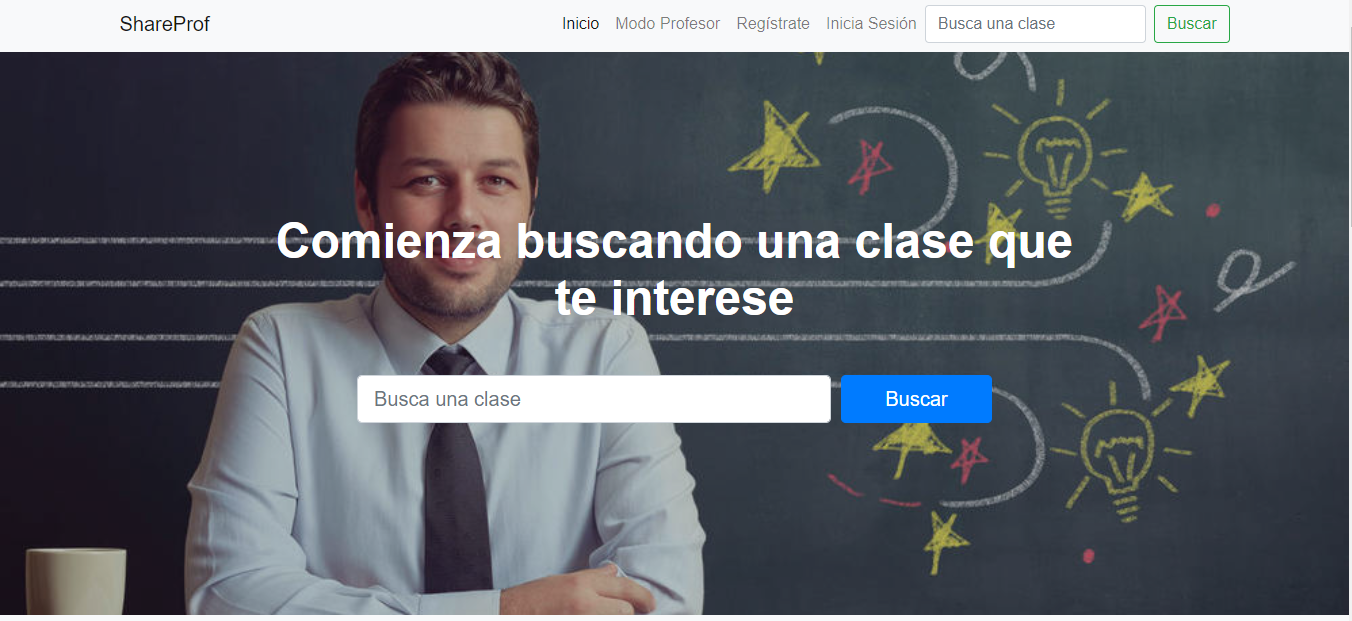
\includegraphics[scale=0.4]{usos/cap1.png}
    \caption{Pantalla de inicio}
    %\label{fig:my_label}
\end{figure}

\begin{figure}
    \centering
    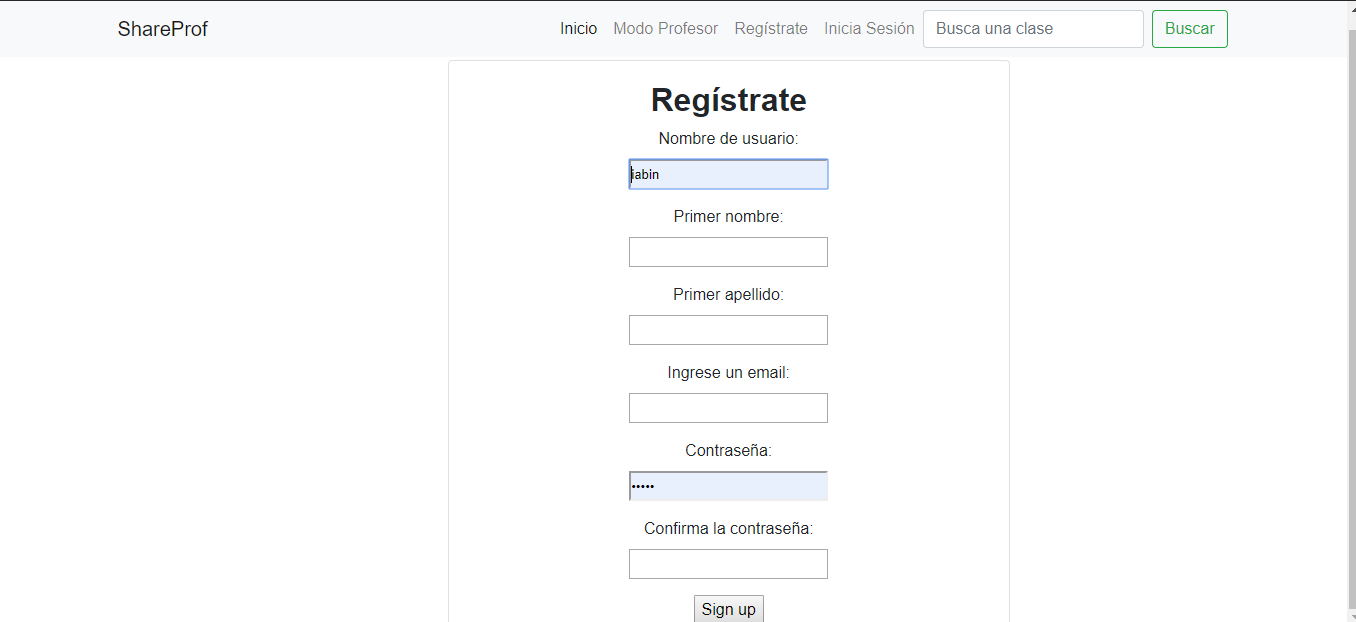
\includegraphics[scale=0.4]{usos/registro.png}
    \caption{Pantalla de registro}
    %\label{fig:my_label}
\end{figure}

\begin{figure}
    \centering
    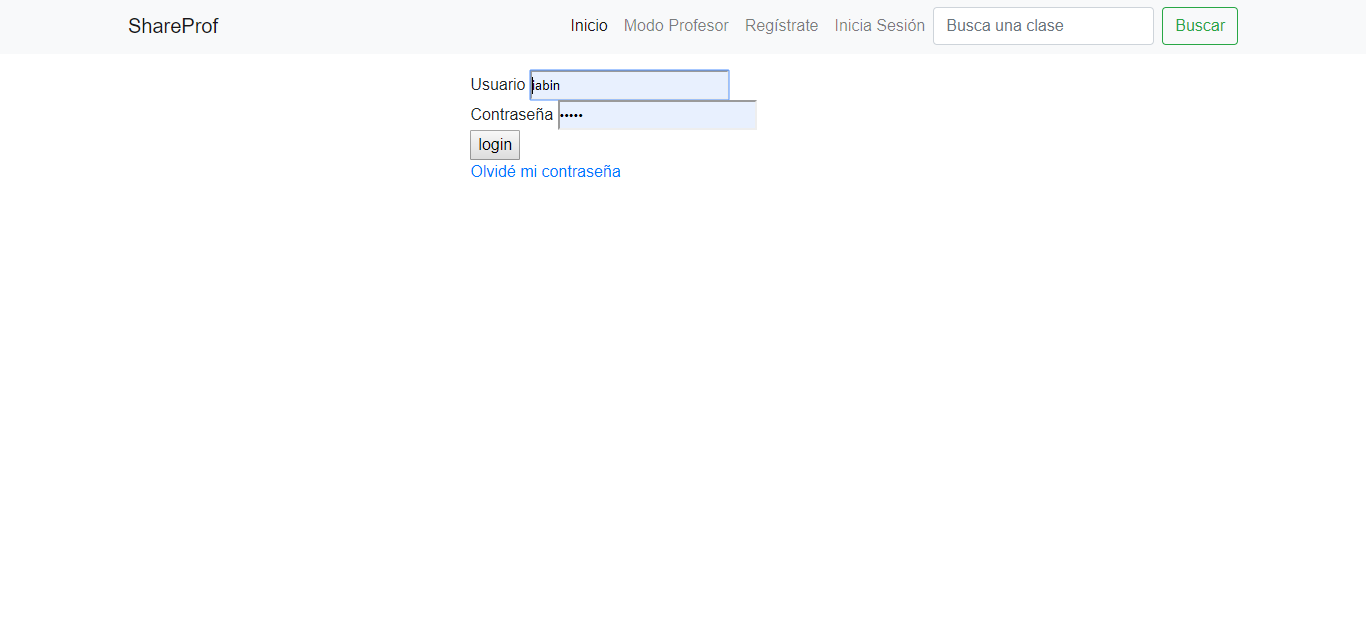
\includegraphics[scale=0.4]{usos/login.png}
    \caption{Pantalla de login}
    %\label{fig:my_label}
\end{figure}

\begin{figure}
    \centering
    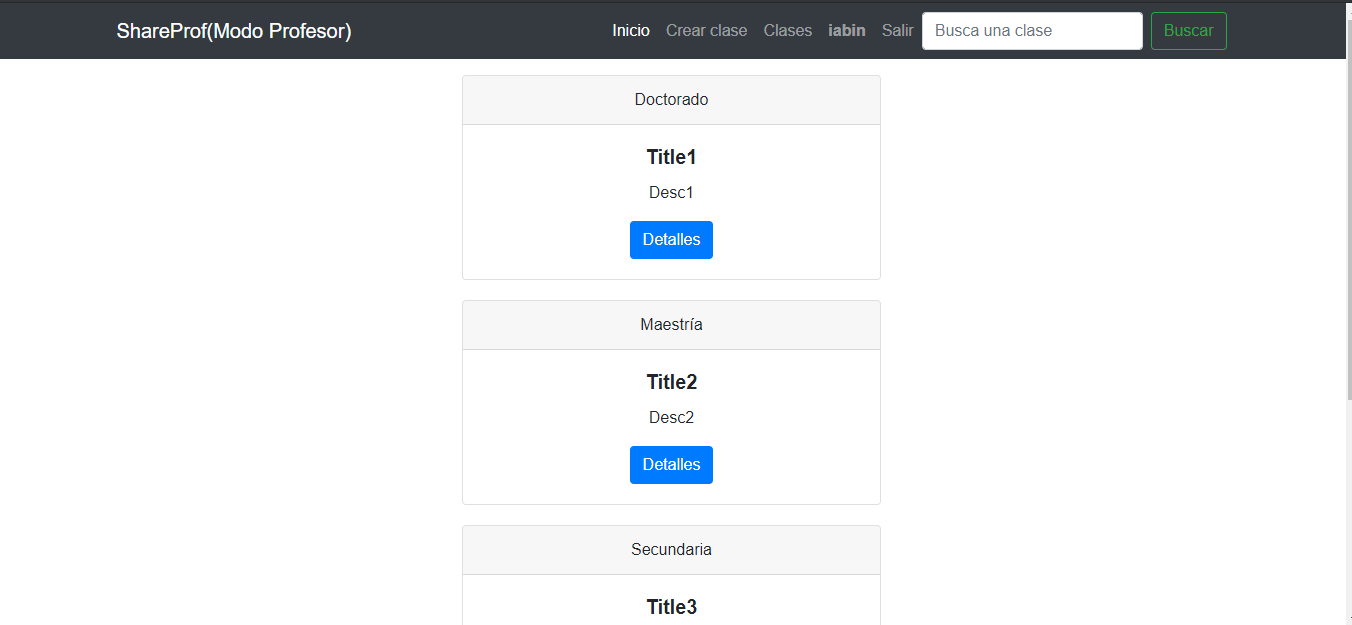
\includegraphics[scale=0.4]{usos/modoProf.png}
    \caption{Pantalla de modo profesor}
    %\label{fig:my_label}
\end{figure}

\begin{figure}
    \centering
    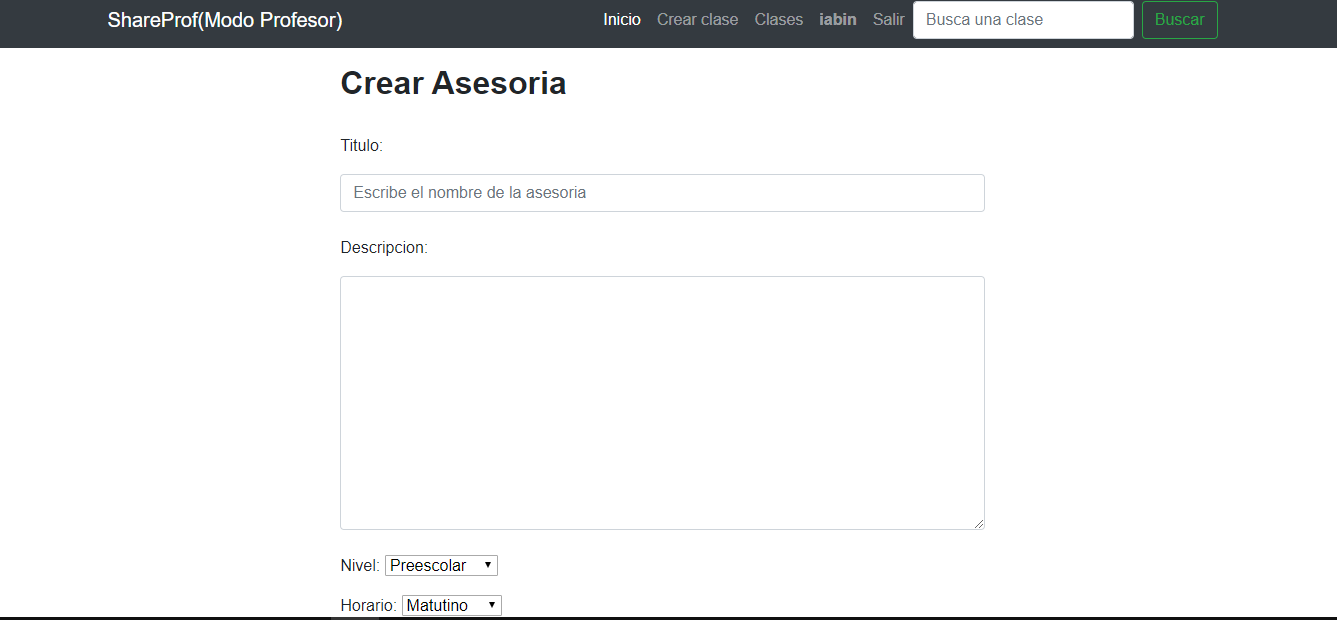
\includegraphics[scale=0.4]{usos/crear.png}
    \caption{Pantalla de crear nueva clase}
    %\label{fig:my_label}
\end{figure}
\newpage
\section{Comentarios}
Fue un proyecto largo ya que debíamos de hacer una variedad de cosas, pero fue divertido y nos dejó mucho aprendizaje. \\\\% el salmo <3 
Tuvimos al principio algunos problemas, ya que habíamos hecho las EC2 antes de hacer las subredes. además de que al principio nuestro servidor web no tenía internet. Estaba mal configurado el internet gateway. nos tardamos un buen rato con eso.\\\\
El servidor de email también en especial fue complicado, debido a que hay que hacer configuraciones muy específicas.\\\\
De igual manera el servidor de aplicación, debías comprender a fondo que es lo que pasaba en la VPC para poder desplegarlo de manera correcta.\\\\
Al final hicimos los toques necesarios para terminar de configurar el servidor web y todo quedó muy bien.
\end{document}

